\subsection{Admin Dashboard Implementation}
The administrative dashboard provides a secure, centralized interface for authorized personnel to monitor, manage, and configure platform resources, including user directories, project states, workflow executions, and generated system files. It employs a standardized layout architecture with dedicated state management and filtered pagination routines.

\subsubsection{RequireAdmin Guard}

\textbf{Purpose:} Acts as a strict route-level security barrier, ensuring only authenticated users possessing the explicit "ADMIN" role designation can access the dashboard sub-routes.

\vspace{0.2cm}
\noindent\textbf{Location:} \texttt{src/pages/admin/RequireAdmin.jsx}

\vspace{0.2cm}
\noindent\textbf{Notes:}
\begin{itemize}
    \item Intercepts navigation requests by examining the \texttt{userDetails.role} property extracted from the global \texttt{UserContext}.
    \item Suspends redirection and renders null while client cookies and session states are still actively loading to prevent layout flashing.
    \item Unauthenticated users are force-routed to \texttt{/login}, while standard users attempting unauthorized access are safely redirected to the \texttt{/overview} dashboard.
\end{itemize}

\begin{lstlisting}
import { useContext } from "react";
import { Navigate, Outlet } from "react-router-dom";
import { User } from "../../context/UserContext";

export default function RequireAdmin() {
  const { auth, loading } = useContext(User);

  if (loading) return null;

  const isLoggedIn = !!auth?.accessToken;
  const role = auth?.userDetails?.role;

  if (!isLoggedIn)        return <Navigate to="/login"    replace />;
  if (role !== "ADMIN")   return <Navigate to="/overview" replace />;

  return <Outlet />;
}
\end{lstlisting}

\subsubsection{AdminLayout Component}

\textbf{Purpose:} Defines the structural shell of the administrative interface, encompassing a persistent top navigation header, a dedicated side navigation menu, and a dynamic content rendering area.

\vspace{0.2cm}
\noindent\textbf{Location:} \texttt{src/pages/admin/AdminLayout.jsx}

\vspace{0.2cm}
\noindent\textbf{Components Used:}
\begin{itemize}
    \item \texttt{AdminSidebar} --- Fixed left-hand navigation component mapping to internal administrative modules.
    \item \texttt{Outlet} --- React Router component serving as the dynamic injection point for nested administrative page content.
\end{itemize}

\vspace{0.2cm}
\noindent\textbf{Notes:}
\begin{itemize}
    \item Extracts the active administrator's profile from \texttt{UserContext} to dynamically compute and render an avatar icon utilizing their first and last initials.
    \item Exposes a topbar interface that includes quick-access routing back to the main \texttt{/overview} page and user profile settings.
\end{itemize}

\subsubsection{AdminSidebar Component}

\textbf{Purpose:} Renders the primary navigation links for the admin dashboard alongside global session termination controls.

\vspace{0.2cm}
\noindent\textbf{Location:} \texttt{src/pages/admin/components/AdminSidebar.jsx}

\vspace{0.2cm}
\noindent\textbf{Notes:}
\begin{itemize}
    \item Maps over a hardcoded \texttt{NAV} constant to render active-state aware \texttt{NavLink} elements for Users, Projects, Executions, and Node Files.
    \item Mounts an explicit \texttt{handleLogout} event handler that purges \texttt{accessToken}, \texttt{refreshToken}, and \texttt{userDetails} from browser \texttt{js-cookie} storage before wiping the global context and routing to \texttt{/login}.
\end{itemize}

\subsubsection{Main Users Directory Page}

\textbf{Purpose:} Renders a comprehensive, paginated table of all registered platform users, empowering administrators to filter records, mutate user roles, and execute account deletions.

\vspace{0.2cm}
\noindent\textbf{Route:} \texttt{/admin/users}

\vspace{0.2cm}
\noindent\textbf{Components Used:}
\begin{itemize}
    \item \texttt{RoleBadge} --- Contextual visual indicator mapping "ADMIN", "USER", and "EDITOR" roles to distinct CSS classes.
    \item \texttt{StatusCell} --- Composite badge rendering email verification status ("Verified" vs "Pending") alongside account disablement flags.
    \item \texttt{DeleteModal} --- Overlay confirming destructive user deletion actions.
    \item \texttt{RoleModal} --- Interface overlay to reassign system roles via a select dropdown.
\end{itemize}

\vspace{0.2cm}
\noindent\textbf{Notes:}
\begin{itemize}
    \item Maintains internal state for pagination limits (10, 25, or 50 rows) and filters, automatically resetting the page index to zero whenever a filter or limit parameter is modified.
    \item Executes \texttt{getUsers()} from the \texttt{adminService}, passing dynamic search parameters (email, name, role, verification status) alongside pagination \texttt{skip} and \texttt{limit} variables.
    \item Implements an over-fetching strategy (\texttt{limit + 1}) to seamlessly detect the existence of subsequent pages without requiring total count aggregation from the backend API.
    \item Dispatches administrative network requests to update roles via \texttt{updateUserRole()} and remove users via \texttt{deleteUser()}, triggering immediate refetch cycles upon successful resolution.
\end{itemize}

\begin{lstlisting}
const fetchUsers = useCallback(async () => {
    setLoading(true);
    setError(null);
    try {
      const params = {
        skip: page * limit,
        limit: limit + 1,   // fetch one extra to detect next page
        role:       roleFilter || undefined,
        isVerified: verFilter  !== "" ? verFilter : undefined,
      };
      if (search) {
        if (search.includes("@")) params.email = search;
        else params.firstName = search;
      }
      const json = await getUsers(params, setAuth);
      const raw  = json?.data ?? [];
      setHasMore(raw.length > limit);
      setUsers(raw.slice(0, limit));
    } catch (e) {
      setError(e.message);
    } finally {
      setLoading(false);
    }
  }, [page, limit, roleFilter, verFilter, search, setAuth]);
\end{lstlisting}

\begin{figure}[H]
    \centering
    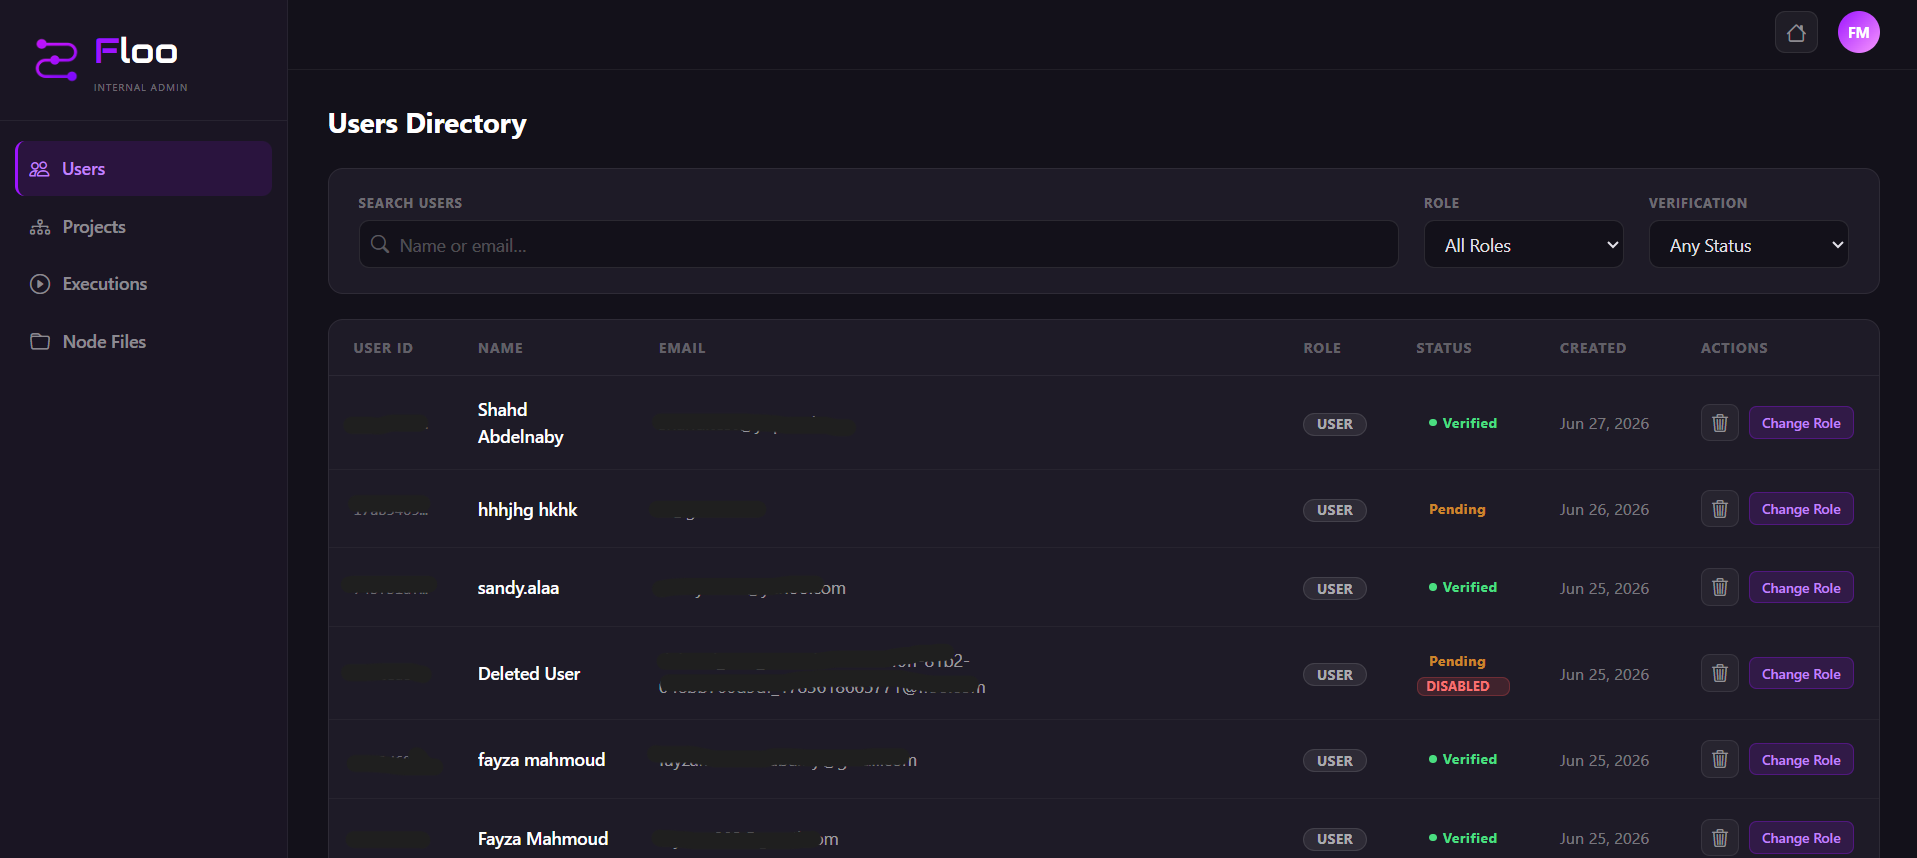
\includegraphics[width=0.95\textwidth]{images/admin-dashboard/admin-users-image.png}
    \caption{Main Users Directory Page Image}
\end{figure}

\subsubsection{Main Projects Management Page}

\textbf{Purpose:} Provides a high-level table view of user-generated workflow projects across the system, allowing filtering by active state and project type.

\vspace{0.2cm}
\noindent\textbf{Route:} \texttt{/admin/projects}

\vspace{0.2cm}
\noindent\textbf{Notes:}
\begin{itemize}
    \item Utilizes an isolated \texttt{ProjectModal} view to expose granular database properties including Version ID, Trigger counts, Description, and an array of individual Node labels attached to the underlying workflow.
    \item Maps custom project types ("Personal", "Team", "Public") through dynamic visual indicators alongside Active/Inactive toggles.
    \item Implements client-side filtering arrays to search across Project IDs and Names over the locally fetched paginated data blocks.
\end{itemize}

\begin{figure}[H]
    \centering
    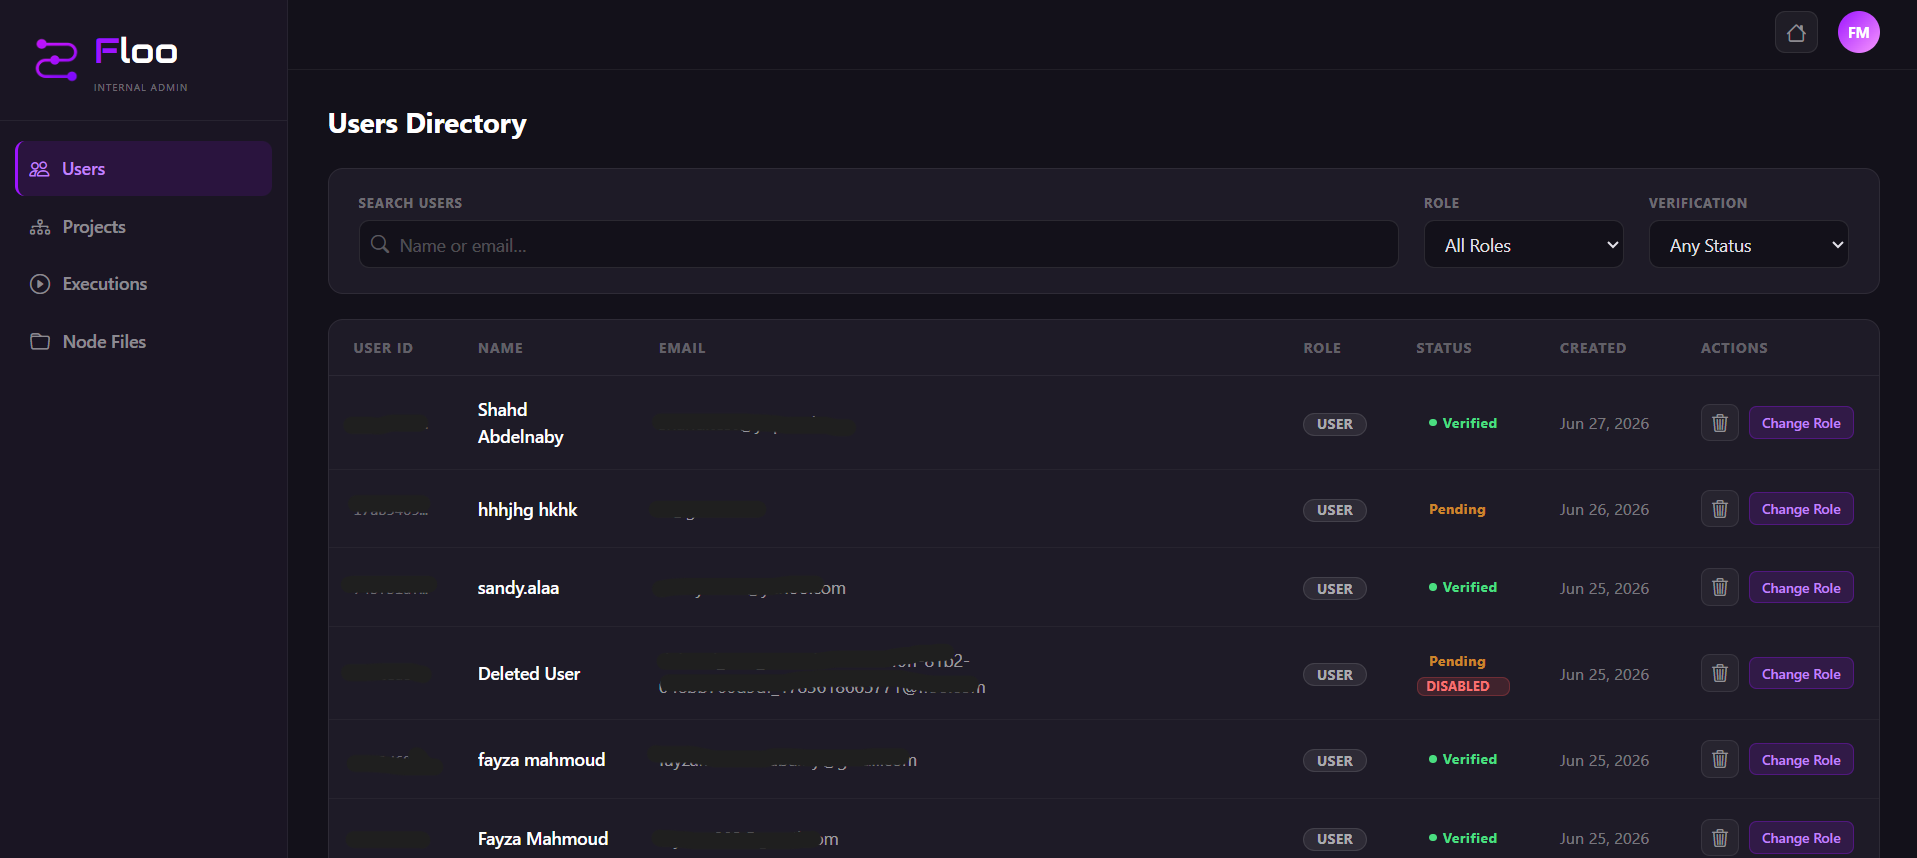
\includegraphics[width=0.95\textwidth]{images/admin-dashboard/admin-users-image.png}
    \caption{Main Projects Management Page Image}
\end{figure}

\subsubsection{Main Executions Log Page}

\textbf{Purpose:} Exposes historical and active workflow run logs across the entire platform ecosystem, visualizing duration, terminal states, and raw JSON outputs.

\vspace{0.2cm}
\noindent\textbf{Route:} \texttt{/admin/executions}

\vspace{0.2cm}
\noindent\textbf{Notes:}
\begin{itemize}
    \item Mounts a sophisticated \texttt{StatusBadge} mapper evaluating "SUCCESS", "CANCELED", "RUNNING", "TIMEOUT", and "ERROR" states, appending CSS animations (pulsing dots) for active tasks.
    \item Computes execution lifecycles dynamically using a \texttt{duration()} utility function that diffs the \texttt{startedAt} and \texttt{endedAt} ISO strings into human-readable HH:MM:SS formats.
    \item Encapsulates execution payloads inside an \texttt{OutputModal}, actively attempting to \texttt{JSON.parse()} the output string to render it inside a beautifully formatted, scrollable \texttt{<pre>} block, gracefully falling back to raw text on failure.
\end{itemize}

\begin{figure}[H]
    \centering
    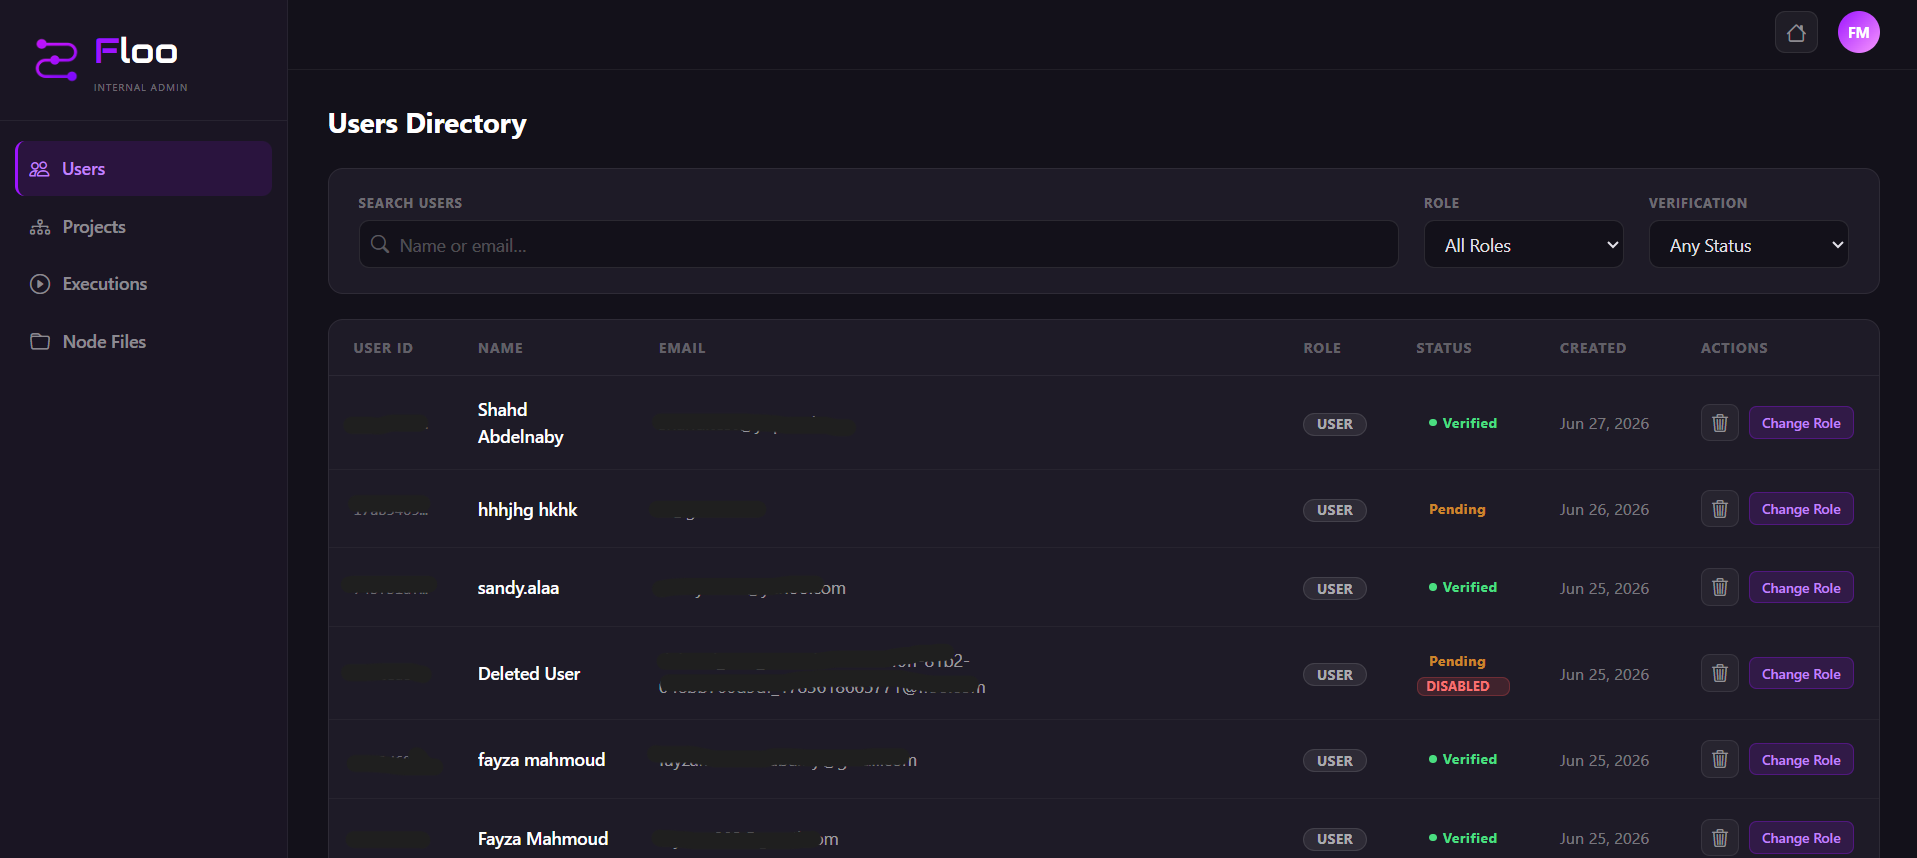
\includegraphics[width=0.95\textwidth]{images/admin-dashboard/admin-users-image.png}
    \caption{Main Executions Log Page Image}
\end{figure}

\subsubsection{Main Node Files Page}

\textbf{Purpose:} Catalogs underlying file blobs and digital assets generated or ingested by workflow nodes, presenting inline previews for imagery and deep-links for file downloads.

\vspace{0.2cm}
\noindent\textbf{Route:} \texttt{/admin/node-files}

\vspace{0.2cm}
\noindent\textbf{Notes:}
\begin{itemize}
    \item Features a robust \texttt{getMimeLabel} and \texttt{getMimeIcon} factory architecture that translates raw \texttt{mimeType} strings into clean UI indicators (e.g., mapping \texttt{application/json} to the \texttt{bi-filetype-json} Bootstrap icon).
    \item Instantiates a specialized \texttt{FileModal} configured to intercept \texttt{image/*} mime types and render inline \texttt{<img>} previews directly inside the administrative panel.
    \item Securely maps external asset URLs utilizing \texttt{target="\_blank"} and \texttt{rel="noreferrer"} anchors to prevent security leakages when navigating to raw blob endpoints.
\end{itemize}

\begin{figure}[H]
    \centering
    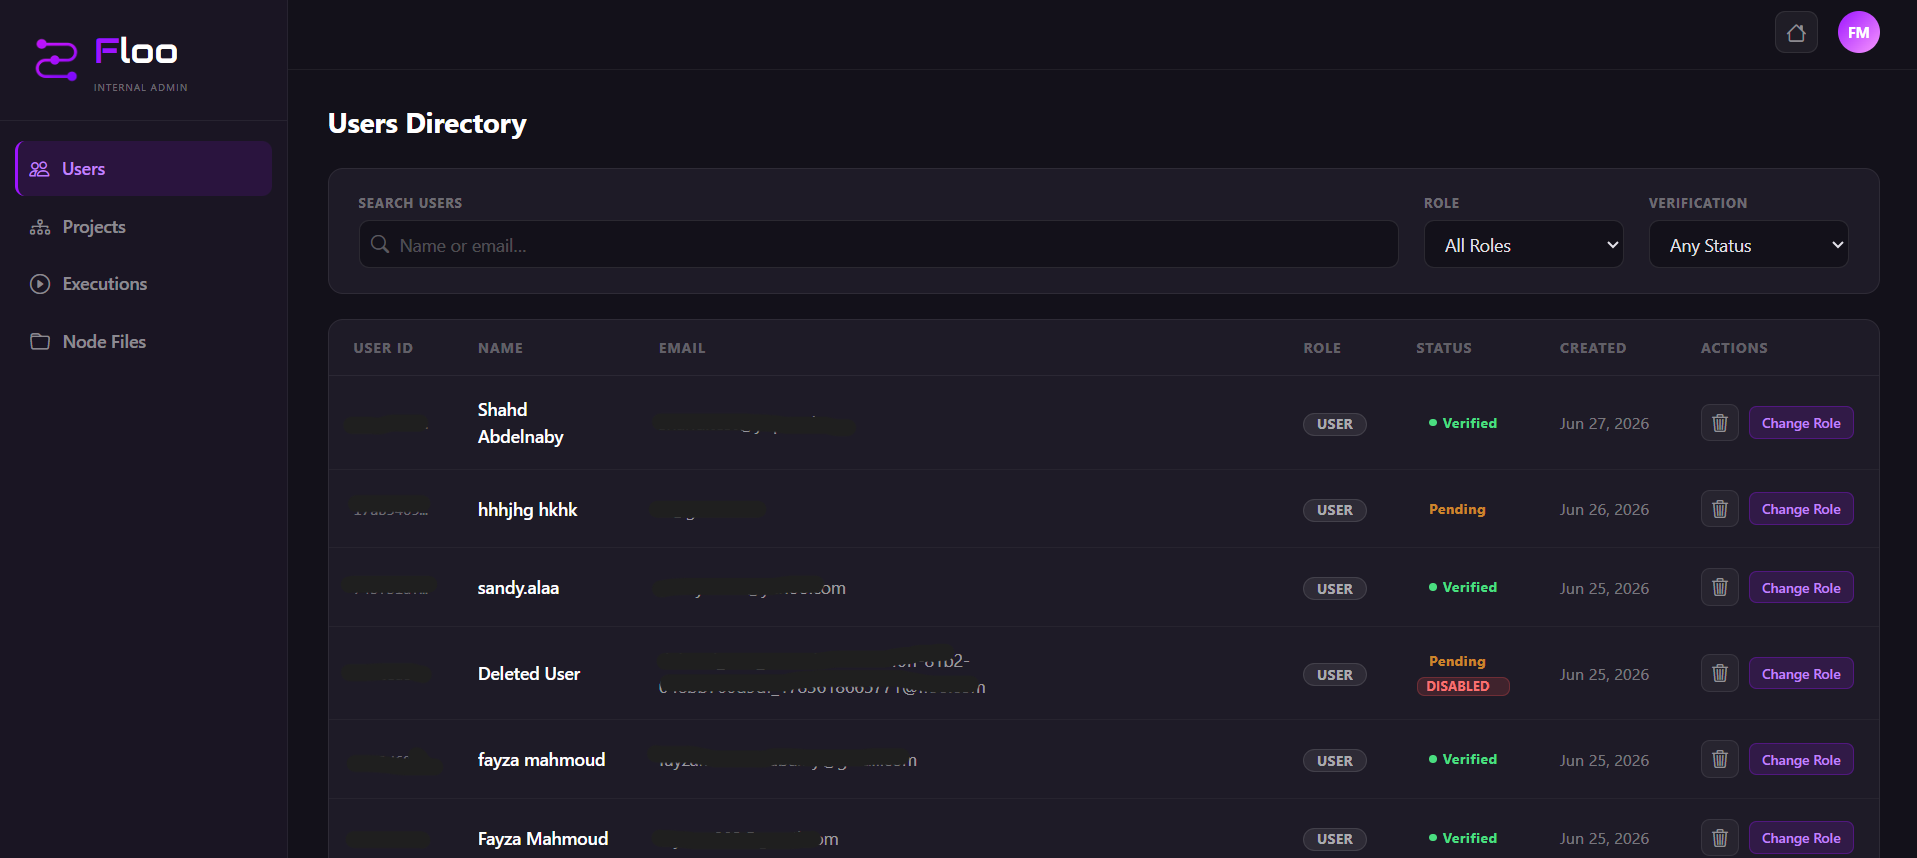
\includegraphics[width=0.95\textwidth]{images/admin-dashboard/admin-users-image.png}
    \caption{Main Node Files Page Image}
\end{figure}

\subsubsection{Admin API Services Layer}

\textbf{Purpose:} Standardizes administrative backend communications by exporting dedicated asynchronous fetch closures wrapped in the protected \texttt{FetchWithAuthService} layer.

\vspace{0.2cm}
\noindent\textbf{Location:} \texttt{src/pages/admin/adminService.js}

\vspace{0.2cm}
\noindent\textbf{Methods Configuration:}
\begin{table}[htbp]
\centering
\caption{Administrative API Service Methods}
\label{tab:admin-api-methods}
\begin{tabular}{|p{3.5cm}|p{2cm}|p{7.5cm}|}
\hline
\textbf{Function Method} & \textbf{HTTP} & \textbf{Parameter Handling} \\
\hline
\texttt{getUsers} & GET & Constructs \texttt{URLSearchParams} mapping \texttt{role}, \texttt{isVerified}, \texttt{email}, \texttt{skip}, and \texttt{limit} keys. \\
\hline
\texttt{deleteUser} & DELETE & Passes targeting \texttt{id} directly inside the URL path parameter. \\
\hline
\texttt{updateUserRole} & PATCH & Stringifies a JSON payload encapsulating the modified \texttt{role} property. \\
\hline
\texttt{getProjects} & GET & Appends \texttt{active}, \texttt{type}, \texttt{skip}, and \texttt{limit} query strings for targeted data retrieval. \\
\hline
\texttt{getExecutions} & GET & Applies base \texttt{skip} and \texttt{limit} queries to the \texttt{/execution/all} backend endpoint. \\
\hline
\texttt{getNodeFiles} & GET & Relies on offset pagination parameters fetched via \texttt{/node/files/all}. \\
\hline
\end{tabular}
\end{table}